\documentclass[bigger]{beamer}
\setbeameroption{show only notes}
\setbeamercolor{note page}{bg=white}
\setbeamercolor{note title}{bg=white}

\setbeamersize{text margin left=1cm, text margin right=1cm}
\setbeamertemplate{navigation symbols}{}
\setbeamertemplate{itemize items}{\textbullet}

\usepackage{graphicx}
\usepackage{helvet}
\renewcommand{\familydefault}{\sfdefault} % Sans-serif font like Arial
\setbeamerfont{frametitle}{size=\LARGE}
\setbeamerfont{framesubtitle}{size=\Large}
% \setbeamerfont{note page}{size=\footnotesize}

% \usebackgroundtemplate%
% {%
%   
\includegraphics[width=\paperwidth,height=\paperheight]{images/test_card.jpg}%
% }
        
\begin{document}
\title{All Code Sucks}
\subtitle{Why Bad Code is Everywhere and What to Do About It}

\author{Joe J Collins \\
  \href{mailto:j.collins@zengenti.com}{j.collins@zengenti.com} \\
  \href{https://linkedin.com/in/joejcollins}{linkedin.com/in/joejcollins}
}

\institute{
\includegraphics[height=1.5cm]{images/zengenti.png}}

\date{\today}
\date{21 March 2024}

\begin{frame}
  \titlepage
  \note{I'm Joe Collins, I'm from Zengenti.\\
  We do websites for universities and local authorities.\\
  I don't actually do any websites, I work in the hosting team.\\
  We maintain the cloud on which the websites run.\\
  We use a combination of Ansible and Python\\
  to maintain an estate of about 3000 servers.\\
  However, tonight Matthew,\\
  I am going to talk about why all code sucks.\\
  \vfil
  We all know what good code looks like,\\
  or at least we think we do.\\
  But I should probably define what I mean by sucky code.\\}
\end{frame}


\begin{frame}{What is sucky code?}
  \framesubtitle{}
  \begin{quote}
    ``Programs are meant to be read by humans and
    only incidentally for computers to execute.''\\
    \hfill --- Donald Knuth
  \end{quote}
  \bigskip
  \begin{quote}
    ``It is better to have clean code that doesn't work 
    than crap code that does.''\\
    \hfill --- Robert C. Martin
  \end{quote}
  \note{Don't take my word for it,\\
  Donald Knuth the Yoda of Computer Science\\
  says that code is for humans to read\\
  and sometimes for computers to run.\\
  He is all about the readability.\\
  \vfil
  Uncle Bob Martin in his inimitable style\\
  backs this up but uses the term clean code.\\
  But it is really a proxy for readability.\\
  If you and understand it then you can fix it,\\
  but if you can't understand it and it breaks you can't fix it.
  }
\end{frame}

\begin{frame}{The Great Hunt for Non Sucky Code}
  
\includegraphics[width=\textwidth]{images/companies.png}
  \note{I have been at this for about 25 years.\\
  Looking for code that doesn't suck.\\
  Trying to produce code that doesn't suck.\\
  I have worked with scumbags and saints.\\
  And in companies big and small.\\
  But all the code sucked.  Consistently.\\
  We did amazing things with it.  But it still sucked.
  \vfil
  Maybe I was just unlucky.\\
  But I have come to the conclusion that all code sucks.\\
  And that I should stop looking for the perfect code.\\
  And instead admit that all code sucks.\\
  And then work out what to do about it.}
\end{frame}

\begin{frame}{Why Code Sucks}
  \framesubtitle{The statistics favour of suck}
  \begin{itemize}
    \item Half of everything is below average
    \pause
    \item Sturgeon's Revelation (90\% of everything is shit)
    \pause
    \item The 2 Year Old Programmer Problem (inexperience)
  \end{itemize}
  \note<1>{
    Straight out of the gate, half of everything it below average.\\
    Well below the median.\\
    You don't have to be Francis Galton to realize that.}
    \vfil
    \note<2>{Then there is Sturgeon's law or revelation\\
    or whatever you want to call it.\\
    He was talking about science fiction at the time\\
    but it works in this situation.\\
    Only some things are really good.\\
    Put another way most stuff isn't that good.}
    \note<3>{
    Then an issue particular to the programming business,\\
    the demand for programmers over the last 25 years has always outstripped supply.\\
    When I started working the average working age was 2 years.\\
    And that hasn't changed.\\
    As more and more people have entered the business\\
    then have kept the average age down.\\
    As a group we still don't have that much experience.
    }
\end{frame}

\begin{frame}{Why Code Sucks}
  \framesubtitle{Organisations tend to suck}
  \begin{itemize}
    \item Structure of Software Startups (early school leaver syndrome)
          \pause
    \item Summer Student Projects (unsupervised use of new technology)
          \pause
    \item Prototypes in Production (commercial imperative)
          \pause
    \item Agile (as an excuse for sucky code)
          \pause
    \item New projects = New programmers (NASA example)
  \end{itemize}
  \note<1>{
    Startups are the worst}
    
\end{frame}

\begin{frame}{Why Code Sucks}
  \framesubtitle{Psycho Suck}
  \begin{itemize}
    \item Availability bias (you only ever look at the bad code)
    \pause
    \item The Illusion of Explanatory Depth (everything is simple until you look)
    \pause
    \item Parkinson's Law of Triviality (judging software design=nuclear reactor)
    \pause
    \item The Lake Wobegon Effect (we all think we are above average)
  \end{itemize}
\end{frame}

\begin{frame}{What Not To Do}
  \framesubtitle{}
  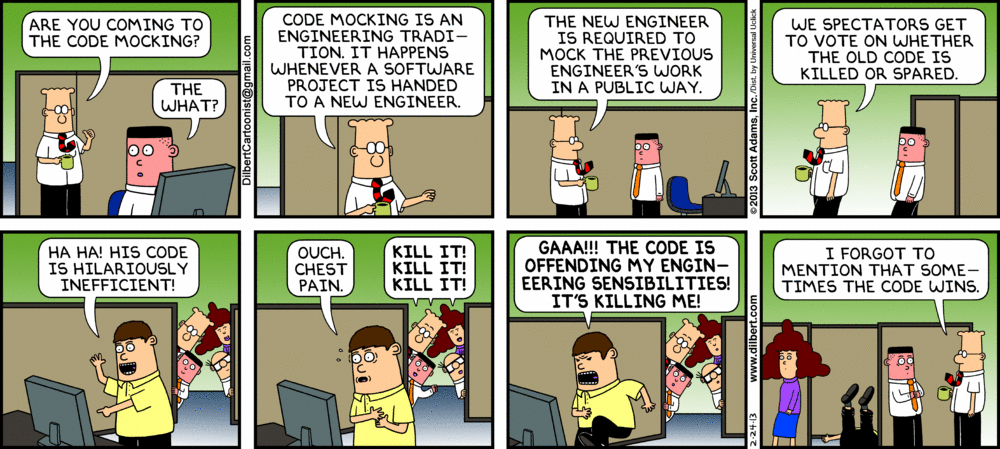
\includegraphics[width=\textwidth]{images/code-mocking.png}
\end{frame}

\end{document}
